\setlength{\baselineskip}{20pt}
\chapter{大规模停车位数据集构建与半监督检测框架}
\label{cha:chap2}

\section{研究动机}
自动泊车技术在自动驾驶领域占据着不可或缺的重要地位。精准的停车位检测作为自动泊车系统的关键起始环节，对后续车辆规划有着直接影响。在此情形下，环视摄像头系统成为首选解决方案，它能够提供车辆周围环境的全景鸟瞰图，从而更高效地实现停车位检测。传统停车位检测方法严重依赖手工提取的特征，诸如拐角与线条等，这些方法远不能达到令人满意的精度，特别是在几何特征匮乏的场景中。 

随着各类基于深度学习的目标检测技术不断发展，基于学习的停车位检测算法如今已取代传统方法。首个基于学习的算法DeepPS\cite{zhang2018vision}及其基准数据集ps2.0的问世，极大地推动了该领域的进步。此后，研究人员通过标记点回归\cite{huang2019dmpr}、图神经网络GNN\cite{min2021attentional}以及基于Transformer的方法\cite{bui2023transformer}等多种途径，致力于提升检测精度。近期，这些算法在基准数据集ps2.0上取得了先进性能，查准率超99\%。然而，现实停车场景往往更为复杂棘手。当这些解决方案应用于实际自动泊车场景时，常常难以达到预期性能。因此，构建一个规模更大、挑战性更强且更贴合实际的数据集迫在眉睫，这对于推进实际停车位检测以及完善算法可行性评估意义重大。 

为满足上述需求，本文收集并标注了一个大规模真实场景数据集，命名为CRPS-D\cite{zhang2025advancing}，用于车位检测任务。该数据集涵盖地上停车场、地下停车建筑、路边停车区等多种车位类型，旨在囊括城市环境中各类真实泊车场景。数据采集覆盖不同时间段及各种天气条件，如白天、黑夜、晴天、阴天与雨天。据本文所知，该数据集在规模上远超所有公开数据集（如ps2.0\cite{zhang2018vision}和SNU\cite{do2020context}）。此外，相较于这些数据集，CRPS-D具有更高的车位集中度、更多的斜向车位示例以及更复杂的道路场景。这些因素共同提升了车位检测的复杂度，提供了一个全面且极具挑战性的基准，有力推动真实场景下车位检测技术的发展。 

另一方面，本文观察到在真实场景中，停车位检测方法的性能在很大程度上取决于训练数据的规模与多样性。然而，停车位作为典型的结构化目标，其标注过程通常涉及多个关键点及其结构关系，标注成本高、周期长，导致现有公开数据集在规模和场景覆盖方面普遍存在欠缺。这使得基于全监督学习的停车位检测方法在面对复杂光照、多视角变化以及非标准停车形式时，泛化能力明显受限。 

为缓解标注数据受限对模型训练的影响，近年来半监督学习在目标检测等任务中逐渐受到关注。通过引入未标注数据参与模型训练，半监督学习能在一定程度上降低对人工标注的依赖。然而，停车位检测任务因目标结构复杂、关键点分布稀疏，致使半监督学习方法在此任务中的应用仍面临较大挑战，如何在保证检测稳定性的同时有效利用未标注数据，尚缺乏系统性研究。 

为解决这一问题，本文提出了首个停车位检测半监督范式。该范式基于教师-学生（Teacher-Student）框架\cite{tarvainen2017mean}，并集成定制化的置信度引导掩码（CGM）一致性约束以及自适应特征扰动机制（Adaptive-VAT）。具体而言，教师模型是学生模型的指数移动平均（EMA），通过一致性正则化引导学生模型学习。然而，强制潜在错误预测保持一致可能产生负面影响。为缓解此问题，本文提出使用可训练的置信度图为不同区域分配不同权重，并遮蔽（Mask）低置信度区域。该方法为无标签数据构建了一种置信度引导的掩码一致性约束。 

此外，考虑到教师-学生模型的目标是促使学生模型在不同扰动下产生稳定输出，本文设计了Adaptive-VAT，一种自适应选择性特征扰动机制，用以生成更强大且合理的对抗噪声。本文的Adaptive-VAT会依据教师或学生模型对扰动的抵抗鲁棒性，选择性地采用其中之一来生成更具挑战性的噪声，从而促进学生模型的有效训练。 

综上所述，本章从数据构建与学习范式设计两方面展开研究： 

（1）一方面，本文构建了CRPS-D数据集，这是一个覆盖多光照、多视角和多停车形式的大规模停车位数据集，为复杂场景下停车位检测方法的研究提供统一的数据基础。该数据集是目前最大的真实世界停车位检测基准数据集。与现有数据集相比，CRPS-D凭借其更大的数据规模、更密集的实例和更具挑战性的场景，有望推动该领域的发展。 

（2）另一方面，结合停车位检测任务特点，本文设计了一种面向停车位检测的半监督检测框架（SS-PSD），通过教师–学生学习范式充分挖掘未标注数据中的潜在信息，为后续结构感知与时序建模方法的研究奠定基础。 

\section{大规模停车位数据集CRPS - D}

\subsection{基本信息}

完整数据集共计包含35379张图像，其中训练图像有29803张，测试图像为5936张。每张图像均对若干标线点及车位进行了标注。标线点的特征通过坐标、形状、类型以及角度来表征，而车位则由这些标线点对确定。图像由安装在侧后视镜的鱼眼摄像头采集，并转化为鸟瞰图；每张分辨率为 $512\times512$ 的环视图覆盖了 $10m\times10m$ 的区域。图\ref{fig_equip}展示了用于数据采集的设备，左侧为主处理设备及四路鱼眼摄像头，右侧呈现的是视野（FOV）的可视化效果。

在训练集与测试集的划分方面，本文实施了最小化数据泄露的策略。具体来讲，本文依据停车场标识、停车区域及采集时段对图像进行分类组织，保证来自同一物理地点的图像不会同时出现在训练集与测试集中。此外，本文数据集包含从视频序列中提取的部分图像；为避免出现近乎重复的样本，本文以较大时间间隔进行抽帧采样。 

\begin{figure}[!h]
\centering
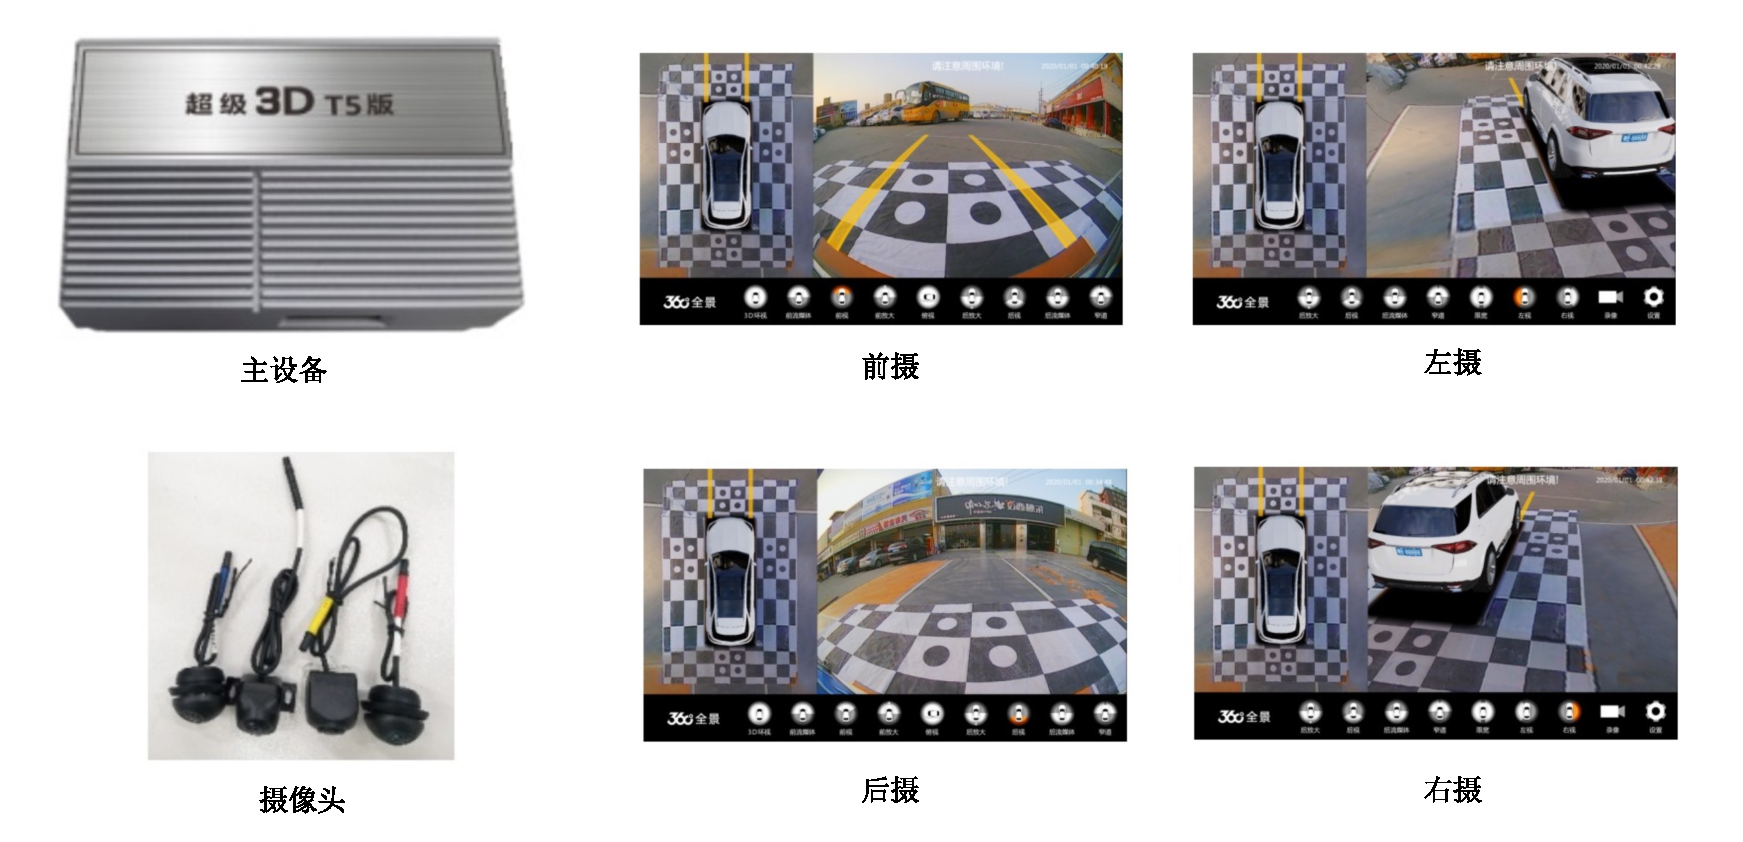
\includegraphics[width=1\textwidth]{figures/chp2/pdf/equip.pdf}
\caption{360度全景环视系统 \\Fig~\ref{fig_equip}~360-degree surround view system}
\label{fig_equip}
\end{figure}


\subsection{定量分析}
在本部分，本文通过深入的数据分析，展现 CRPS-D 数据集相较于现有数据集的显著改进与优势。

\begin{table}[!h]
\centering
\setlength{\tabcolsep}{4.0mm}
\caption{数据规模对比结果 \\Table~\ref{tab_datascale}~Comparison results of data scale}
\begin{tabular}{llccc}
        \toprule
         数据集  & & ps2.0\cite{zhang2018vision} & SNU\cite{do2020context} & \textbf{Ours} \\
        \midrule
             \multirow{3}{*}{总图像数} & 训练集 & 9827 & 18299 & 29803  \\
              & 测试集 & 2338 &	4518	&5936   \\
              & 总数 & 12165	& 22817	& \textbf{35739}  \\
        \midrule
            \multirow{3}{*}{训练集中的车位数}  & 垂直车位 & 9160 & 45610 & 103931  \\
              & 倾斜车位 & 316 &	3276 & 14126   \\
              & 总数 & 9476 & 48886 & \textbf{118057}  \\
        \midrule
             \multirow{3}{*}{测试集中的车位数}   & 垂直车位 & 2087 & 12541 & 21451 \\
              & 倾斜车位 & 81 & 1004 & 2573  \\
              & 总数 & 2168 & 13545 & \textbf{24024}   \\
        \midrule
             总车位数  & 总数 & 11644 & 62431 & \textbf{142081} \\
        \bottomrule
    \end{tabular}
\label{tab_datascale}
\end{table} 

（1）数据规模

数据集规模对于当下的视觉模型（如 SAM\cite{kirillov2023segment}）而言，重要性日益凸显，这也正是本文构建更大规模数据集的原因所在。在图像总数以及车位总数方面，CRPS - D 均实现了数量级的提升。如表\ref{tab_datascale}所示，CRPS-D 数据集的图像总数达 35739 张，分别为 ps2.0 和 SNU 的 2.94 倍与 1.57 倍。尤为突出的是，在总车位数量上，CRPS-D（142081 个）约为 ps2.0（11644 个）的 12.2 倍，为深度神经网络提供了高质量的学习样本。

此外，为进一步衡量数据集的丰富程度，本文计算了“车位-图像密度”（slot-image density），其表达式为：
\begin{equation}
 \mbox{车位图像密度} = \frac{N_{slots}}{N_{images}}
\end{equation}
其中，$N$ 表示不同条件下的样本数量。

在数据集丰富度的横向对比中，CRPS - D 展现出显著的统计优势。特别是其“车位-图像密度”高达 3.98，如表\ref{tab_density} 所示，远高于 ps2.0（0.96）和 SNU（2.74）。这一高密度特征表明，CRPS-D 能够为算法提供更为复杂的空间上下文以及重叠/遮挡样本，促使模型学习更为鲁棒的特征表示，而非简单的模板匹配。这为训练具备更高泛化能力的深度感知网络奠定了坚实的数据基础。 

\begin{table}[!h]
\centering
\caption{车位图像密度 \\Table~\ref{tab_density}~Density of parking slots }
\begin{tabular}{lccccccccc}
\toprule
 & \multicolumn{3}{c}{ps2.0\cite{zhang2018vision}} & \multicolumn{3}{c}{SNU\cite{do2020context}} & \multicolumn{3}{c}{\textbf{Ours}} \\\cmidrule{2-4}\cmidrule{5-7}\cmidrule{8-10}%
 
    & $N_{slots}$ &$N_{images}$ & 密度 & $N_{slots}$ &$N_{images}$ & 密度 & $N_{slots}$ &$N_{images}$ & 密度 \\
\midrule
     训练集 & 9476 & 9827 & 0.96 & 48886 & 18299 & 2.67 & 118057 & 29803 & \textbf{3.96}  \\
    测试集 & 2168 & 2338 & 0.93 & 13545 & 4518 & 3.00 & 24024 & 5936 & \textbf{4.05}  \\
    总数 & 11644 & 12165 & \textbf{0.96} & 62431 & 22817 & \textbf{2.74} & 142081 & 35739 & \textbf{3.98}  \\
\bottomrule
\end{tabular}
\label{tab_density}
\end{table} 



（2）场景分析

为全面覆盖现实世界中的复杂泊车环境，CRPS - D数据集细分为八个特定子集，涵盖“室内弱光 / 强光”、“室外日光 / 雨天 / 阴影 / 夜晚”以及“斜向车位”“受损车位”等多样化场景。如表\ref{tab_sence}所示，相较于基准数据集ps2.0，CRPS-D 在环境广度方面实现了显著突破。它不仅引入了更具挑战性的“室外夜晚”与“受损车位”场景，填补了现有数据集在极端场景下的空白，而且在各细分场景的图像数量级上均有大幅提升。

此外，为直观展现本数据集的优势，本文在图\ref{fig_crpsd}中展示了各场景的示例。从中能够观察到，CRPS-D比ps2.0更贴近现实情况。 


\begin{table}[!h]
\centering
\setlength{\tabcolsep}{1.0mm}
\caption{测试集场景统计信息\\
Table~\ref{tab_sence}~Statistics for the scene data in the test set.}
\begin{tabular}{lccccccccc}
    \toprule
    \multirow{2}{*}{场景} & \multicolumn{2}{c}{室内} & \multicolumn{4}{c}{室外} & \multicolumn{2}{c}{特殊场景} & \multirow{2}{*}{总计} \\
    \cmidrule(lr){2-3} \cmidrule(lr){4-7} \cmidrule(lr){8-9}
    & 弱光 & 强光 & 正常日光 & 雨天 & 阴影 & 夜晚 & 倾斜车位 & 受损车位 & \\
    \midrule
    ps2.0\cite{zhang2018vision} & \multicolumn{2}{c}{226} & 693 & 244 & 1127 & / & 48 & / & 2338 \\
    \textbf{Ours} & 545 & 786 & 1703 & 323 & 1389 & 86 & 802 & 302 & 5936 \\
    \bottomrule
\end{tabular}
\label{tab_sence}
\end{table}


\begin{figure}[!h]
\centering
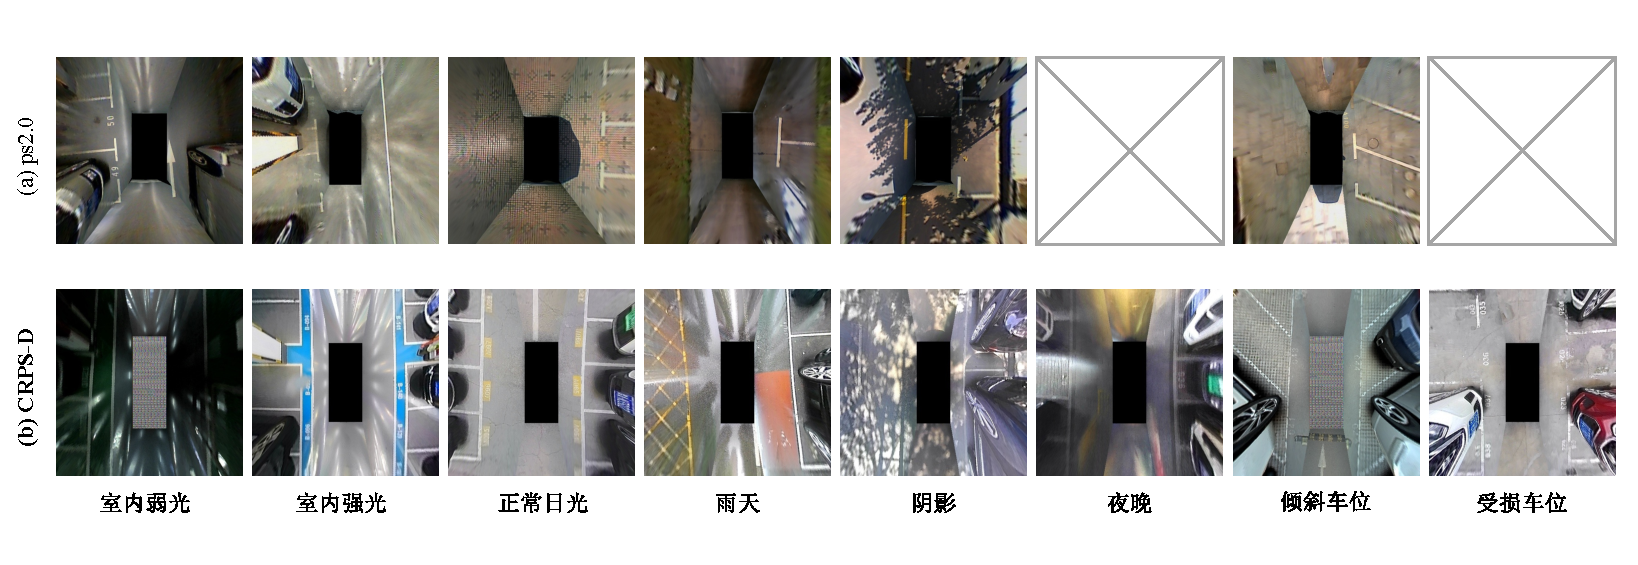
\includegraphics[width=1\textwidth]{figures/chp2/pdf/sence.pdf}
\caption{数据集示例图片 \\Fig~\ref{fig_crpsd}~Example images from the dataset}
\label{fig_crpsd}
\end{figure}

（3）倾斜车位

倾斜式停车位常应用于狭窄街道，旨在更有效地利用道路空间，在现实场景中较为常见。然而，相较于垂直式停车位，倾斜式停车位的检测难度更大，且常被其他数据集忽视。鉴于此，本文提高了倾斜式停车位在数据集中的比例。

倾斜式停车位在狭窄街道频繁使用，以提升道路空间利用率，是现实场景中常见的车位类型。但与垂直车位相比，倾斜车位检测难度更高，且常被其他数据集所忽略。因此，本文特意增加了倾斜车位在数据集中的占比。倾斜车位占比的计算公式如下：
\begin{equation}
 \mbox{倾斜车位比例} = \frac{S_{slant}}{S_{Total}}. 
\end{equation}
其中，$S$ 表示不同类型的停车位样本数量。

如表\ref{tab_slant}所示，本文的CRPS-D数据集包含11.75\%的斜向车位，这一比例显著高于ps2.0（3.41\%）和SNU（6.86\%）。这不仅更真实地反映了现实世界的实际情况，还有助于缓解类别不平衡问题。 

\begin{table}[!h]
\centering
\caption{倾斜停车位占比 \\
Table~\ref{tab_slant}~Proportion of slanted parking slots.}
\begin{tabular}{lccccccccc}
\toprule
 & \multicolumn{3}{c}{ps2.0\cite{zhang2018vision}} & \multicolumn{3}{c}{SNU\cite{do2020context}} & \multicolumn{3}{c}{\textbf{Ours}} \\\cmidrule{2-4}\cmidrule{5-7}\cmidrule{8-10}%
 
    & $S_{slant}$ &$S_{Total}$ & 占比 & $S_{slant}$ &$S_{Total}$ & 占比
    & $S_{slant}$ &$S_{Total}$ & 占比 \\
\midrule
    训练集 & 316 & 9476 & 3.33\% & 3276 & 48886 & 6.70\% & 14126 & 118057 & \textbf{11.97\%}  \\
    测试集 & 81 & 2168 & 3.74\% & 1004 & 13545 & 7.41\% & 2573 & 24024 & \textbf{10.71\%}  \\
    总数 & 397 & 11644 & \textbf{3.41\%} & 4280 & 62431 & \textbf{6.86\%} & 16699 & 142081 & \textbf{11.75\%}  \\
\bottomrule
\end{tabular}
\label{tab_slant}
\end{table} 




\section{半监督停车位检测算法框架}

在本节中，本文将详细阐述SS - PSD架构的构成以及所采用的半监督学习策略。如图\ref{fig_sspsd}所示，整个架构由两个分支构成：学习-学生分支，用于开展模型训练；以及指导-教师分支，在此分支中运用EMA（指数移动平均）以及$M_{\theta}^{S}$的参数来更新$M_{\theta}^{T}$。图中左下部分和右下部分分别对应\textbf{Adaptive - VAT}和\textbf{CGM Consistency}。 

\begin{figure}[!h]
\centering
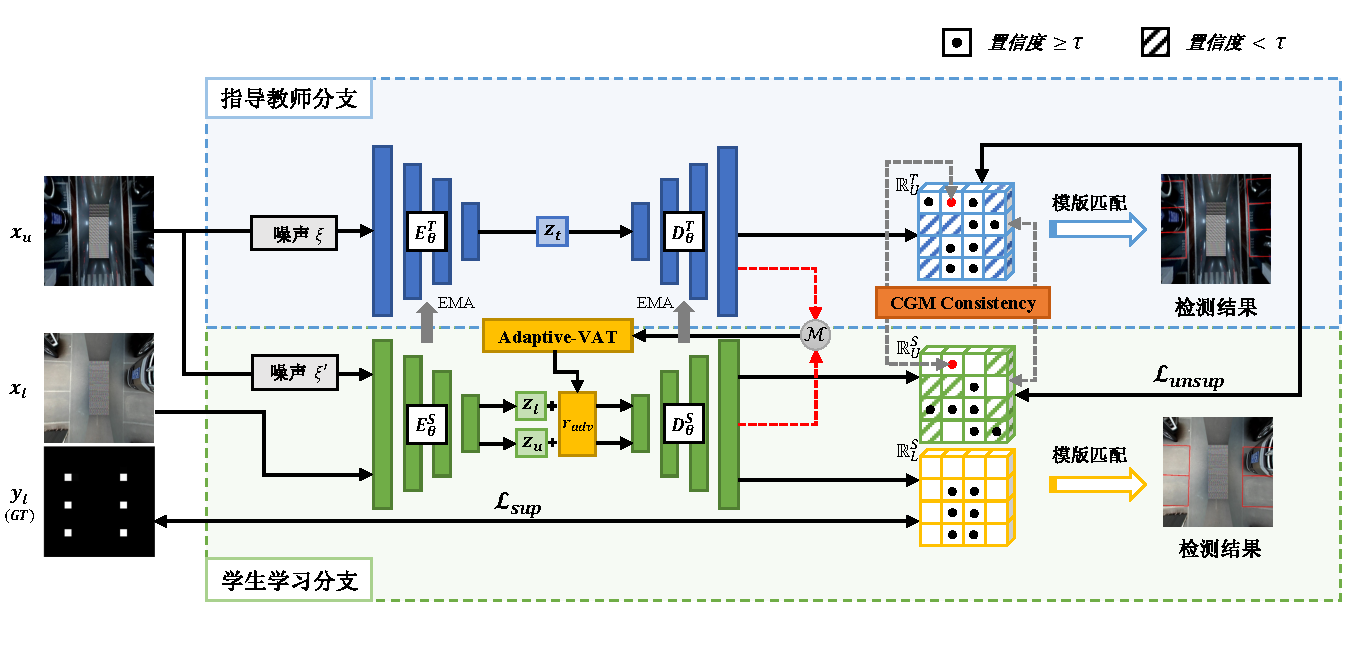
\includegraphics[width=1\textwidth]{figures/chp2/pdf/pipline.pdf}
\caption{SS-PSD的整体架构\\Fig~\ref{fig_sspsd}~Overview of SS-PSD architecture}
\label{fig_sspsd}
\end{figure}

\subsection{问题定义}

首先，本文随机选取一小部分带有对应标签的数据构成有标签数据集，记为\(\mathcal{D}_{L}=\{(\textbf{x}_{l},\textbf{y}_{l})\}\)，而剩余图像则构成无标签数据集\(\mathcal{D}_{U}=\{(\textbf{x}_{u})\}\)。给定一张尺寸为\(512\times512\)的图像\(\textbf{x}_{l}\)及其对应标签\(\textbf{y}_{l}\)，本研究旨在预测一个特征图\(\mathbb{R} \in \mathcal{S}\times \mathcal{S} \times \mathcal{N}\)，其中图像被划分为\(\mathcal{S}\times \mathcal{S}\)个网格。参照DMPR - PS~\cite{huang2019dmpr}的方法，特征图\(\mathbb{R}\)与输入图像中的标线点相对应，\(\mathcal{N}\)个维度代表它们各自的特征。随后，本文应用模板匹配来判定这些点能否构成有效的入口线，进而识别出相应的车位。这一过程可描述如下：

\begin{equation}
\textbf{x}_{l} \xrightarrow{M_{\theta}} \mathbb{R}^{\mathcal{S}\times \mathcal{S} \times \mathcal{N}} \xrightarrow {\text{模版匹配}} \text{停车检测结果}
\end{equation}

其中\(M_{\theta}(\cdot)\)是用于预测标记点的模型，\(\theta\)代表模型参数。
与以往过度依赖昂贵有标签数据集的研究不同，本文利用易于获取的无标签图像\(\textbf{x}_{u}\)来进一步提升性能。 

\subsection{网络架构}

图\ref{fig_sspsd}展示了本文所提出的半监督停车位检测基线模型 (SS - PSD) 的架构，该模型由一个指导教师分支和一个学习学生分支构成。二者具有相同的网络结构，记为\(M_{\theta}=\{E_{\theta}, D_{\theta}\}\)，其中包含编码器\(E_{\theta}: \textbf{x}\rightarrow \textbf{z}\)和解码器\(D_{\theta}: \textbf{z}\rightarrow \mathbb{R}^{\mathcal{S} \times \mathcal{S} \times \mathcal{N}}\)。
具体来讲，本文将教师模型定义为\(M_{\theta}^{T}=\{E_{\theta}^{T}, D_{\theta}^{T}\}\)，学生模型定义为\(M_{\theta}^{S}=\{E_{\theta}^{S}, D_{\theta}^{S}\}\)。

（1）学生分支

本文采用定制的CNN模型~\cite{huang2019dmpr}作为编码器-解码器架构。在学习-学生分支中，编码器\(E_{\theta}^{S}\)同时处理已标注的\(\textbf{x}_{l}\)和未标注的\(\textbf{x}_{u}\)数据，生成潜在特征\(\textbf{z}_{l}\)和\(\textbf{z}_{u}\)，可表示为\(E_{\theta}^{S}(\textbf{x}_{l} / \textbf{x}_{u}) = \textbf{z}_{l} / \textbf{z}_{u}\)。
结合自适应VAT算法生成的对抗噪声\(\textbf{r}_{adv}\)，将\(\textbf{z}_{u}\)和\(\textbf{z}_{l}\)输入解码器\(D_{\theta}^{S}\)，生成最终特征图，可表示为\(D_{\theta}^{S}(\textbf{z}_{l} / \textbf{z}_{u} + \textbf{r}_{adv}) = \mathbb{R}_{L}^{S} / \mathbb{R}_{U}^{S}\)。
所得特征图\(\mathbb{R}\)对应于输入图像中的标记点。随后，本文采用模板匹配方法系统地验证几何关系，判断这些点是否排列成有效的停车位入口线。

（2）教师分支

在此分支中，未标记数据\(\textbf{x}_{u}\)经\(E_{\theta}^{T}\)处理，生成潜在特征\(\textbf{z}_{t}\)，表示为\(E_{\theta}^{T}(\textbf{x}_{u}) = \textbf{z}_{t}\)。然后，该潜在特征被输入到\(D_{\theta}^{T}\)中，生成最终特征图\(\mathbb{R}_{U}^{T}\)，表示为\(D_{\theta}^{T}(\textbf{z}_{t}) = \mathbb{R}_{U}^{T}\)。在训练过程中，本文采用自适应矩估计（Adam）~\cite{kingma2014adam}来最小化\(M_{\theta}^{S}\)的损失函数，同时使用EMA~\cite{tarvainen2017mean}和\(M_{\theta}^{S}\)的参数来更新\(M_{\theta}^{T}\)。 


\subsection{自适应特征扰动}
特征扰动是自监督或半监督学习中广泛采用的策略。在本研究中，并未引入随机噪声，而是借助虚拟对抗训练（VAT\cite{miyato2018virtual}）来估计对抗噪声。该噪声旨在使扰动后预测与原始预测之间的距离最大化。如图\ref{fig_sspsd}左下部分所示，给定分离的潜在特征\(\textbf{z}\)，通过计算梯度引导的对抗噪声\(\textbf{r}\)，让\((D_\theta(\textbf{z}+\textbf{r}) - D_\theta(\textbf{z}))\)达到最大，以此尽可能干扰网络。要达到理想的扰动效果，\(D_\theta\)的模型质量至关重要，因其决定了梯度的搜索方向。

Liu等人\cite{liu2022perturbed}在PS-MT中提出了T-VAT方法，该方法设定\(D_\theta\)为教师模型\(D_{\theta}^{T}\)来计算对抗噪声。但本文认为，这一设定并非总是最优。通过实验观察发现，在特定情形下（尤其是训练初期），学生模型\(D_{\theta}^{S}\)由于受到直接梯度引导，往往表现出更好的特征质量。因此，本文引入了自适应虚拟对抗训练（Adaptive - VAT），以施加最优扰动。该机制依据教师模型和学生模型在生成扰动时的抗扰鲁棒性，自适应地从二者中选择最优的对抗噪声。

具体来讲，Adaptive - VAT不再盲目信赖教师模型生成的扰动方向，而是通过实时评估学生模型与教师模型的确定性强度，动态构建更具挑战性的负样本，如图\ref{fig_sspsd}左下部分所示。这种竞争机制促使学生模型在更为严苛的特征空间内学习稳健的车位几何表征。
为确保原始预测与扰动后预测之间的距离最大化，对抗噪声\(\textbf{r}_{adv}\)综合参考\(D_{\theta}^{T}\)和\(D_{\theta}^{S}\)的响应进行计算，且需满足以下公式：
\begin{equation}
\begin{align}
\text{maximise }& \mathcal{M}\Big(d(D_{\theta}^{T}(\mathbf{z}_l / \mathbf{z}_u) , D_{\theta}^{T}(\mathbf{z}_l / \mathbf{z}_u + \textbf{r}_{adv})), 
&d(D_{\theta}^{S}(\mathbf{z}_l / \mathbf{z}_u), D_{\theta}^{S}(\mathbf{z}_l / \mathbf{z}_u + \textbf{r}_{adv}))
\Big),\\
\text{subject to }& ||\mathbf{r}_{adv}||_2 <=\epsilon,
\end{align}
\end{equation}
其中 $d(\cdot,\cdot)$ 表示均方误差 (MSE) 损失，$\mathcal{M}(\cdot,\cdot)$ 选择 MSE 损失更低的更优解码器。

\subsection{一致性约束}
为构建针对无标签数据的一致性约束，一个直观思路是计算学生模型预测结果\(\mathbb{R}_{U}^{S}\)与教师模型预测结果\(\mathbb{R}_{U}^{T}\)之间的均方误差（MSE\cite{tarvainen2017mean}）损失，以此确保预测的一致性。然而，此方案可能致使潜在的错误预测也被强制保持一致，进而误导网络学习；并且，对特征图\(\mathbb{R}\)中所有网格单元赋予均等权重也并非最优选择。
针对该问题，如图\ref{fig_sspsd}右下部分所示，本文引入置信度图（Confidence Map），为不同的网格单元分配非均衡的注意力，并对低置信度区域进行 Mask。

具体而言，对于特征图\(\mathbb{R} \in \mathcal{S} \times \mathcal{S} \times \mathcal{N}\)，本文将输入图像\(\textbf{x}\)划分为\(16×16\)的网格（即\(\mathcal{S} = 16\)），并设定特征维度\(\mathcal{N} = 9\)（即\(6 + 3\)）。其中，前6个维度遵循DMPR - PS~\cite{huang2019dmpr}的设定，而新增的3个维度用于捕捉检测斜向车位所需的角度及分类细节。也就是说，一个标线点的表征由9个分量构成：用于基准点定位的\((x, y)\)、用于两条边缘角度的\((\cos\theta_{1/2}, \sin\theta_{1/2})\)、标线点形状\(\textbf{s}\)、标线点类型\(\textbf{t}\)（即垂直或斜向）以及置信度\(C\)。

因此，本文最终构建了置信度引导的掩码一致性损失\(\mathcal{L}_{CGM}\)，其表达式为：
\begin{equation}
\begin{cases}
\sum_{i=1}^{\mathcal{S}^{2}} \{ ||C_{i}^{S} - C_{i}^{T}||_2 \} & \text{if } C_{i}^{T} < \tau \\
\sum_{i=1}^{\mathcal{S}^{2}} \{ ||C_{i}^{S} - C_{i}^{T}||_2 + ||q_{i}^{S} - q_{i}^{T}||_2 \times C_{i}^{T} \} & \text{if } C_{i}^{T} \geq \tau
\end{cases}
,
\end{equation}

其中\(q = (x,y,\cos\theta_1,\sin\theta_1,\cos\theta_2,\sin\theta_2,\textbf{s},\textbf{t})\)，下标\(i\)表示\(16×16\)网格中的单元格索引，\(\tau\)为置信阈值（本文设定\(\tau = 0.9\)）。如此一来，本文不仅能够筛选出重要的网格单元格进行监督，还能更加聚焦于那些更有可能包含标记点的网格单元格。 


\subsection{损失函数}
（1）标注数据

对于已标注的图像对 $(\textbf{x}_{l},\textbf{y}_{l})$，可以为预测提供直接的监督。因此，监督损失 $\mathcal{L}_{sup}$ 定义如下：

\begin{equation}
\begin{cases}
\sum_{i=1}^{\mathcal{S}^{2}} \{ ||C_{i}^{S}||_2 \} & \text{if } \textbf{y}_{li} \ 不存在 \\
\sum_{i=1}^{\mathcal{S}^{2}} \{ ||C_{i}^{S} - 1||_2 + ||q_{i}^{S} - \hat{q_{i}}||_2 \} & \text{if } \textbf{y}_{li} 存在
\end{cases}
,
\end{equation}%

其中 $\hat{q_{i}}$ 表示对应的真实值。对于预测而言，(GT) 函数 $\textbf{y}_{li}$ 仅当标记点位于网格单元 $i$ 内时才存在。

（2）未标注数据

对于未标记数据，本文利用 $M_{\theta}^{T}$ 和 $M_{\theta}^{S}$ 之间的置信度引导掩码 (CGM) 一致性来建立无监督约束，如下式所示：

\begin{equation}
\mathcal{L}_{unsup}(\mathcal{D}_{U}, M_{\theta}^{S}, M_{\theta}^{T})=\mathcal{L}_{CGM}
\end{equation}

总目标函数由基于标记数据和未标记数据的两项组成，如下所示：

\begin{equation}
\begin{array}{l}
\mathcal{L}_{total}(\mathcal{D}_{L},\mathcal{D}_{U}, M_{\theta}^{S}, M_{\theta}^{T})= 
\mathcal{L}_{sup}(\mathcal{D}_{L}, M_{\theta}^{S})+ \beta \mathcal{L}_{unsup}(\mathcal{D}_{U}, M_{\theta}^{S}, M_{\theta}^{T})
\end{array}
,
\end{equation}

其中 $\beta=\frac{N_{\mathcal{D}_{U}}}{N_{\mathcal{D}_{L}}}$ 和 $N_{\mathcal{D}_{U}}/N_{\mathcal{D}_{L}}$ 分别表示标记样本和未标记样本的数量。

\section{实验结果及分析}
本节所有实验均在同一硬件平台上进行，具体包括一块 Nvidia 2080Ti GPU（12GB 显存）和一台配备 Intel(R) Xeon(R) E5-2680 v4 @ 2.40GHz 的 CPU 的服务器环境。模型训练使用 PyTorch 框架实现。

\subsection{不同数据划分的结果}

参照Mean Teacher\cite{tarvainen2017mean}方法，本节通过对数据集进行比例抽样来评估所提方法，其中有标签集的比例为\(1/n\)，无标签集的比例为\((1 - \frac{1}{n})\)。针对本文提出的CRPS-D数据集以及公开数据集ps2.0，分别采用\(1/24\)、\(1/12\)、\(1/8\)、\(1/4\)和\(1/2\)的有标签比例进行实验。鉴于本文的SS-PSD是该领域首个半监督解决方案，因此仅能将该方法与现有的公开全监督方案作对比。

（1）CRPS-D

如表\ref{tab_crpsd}所示，在标注比例为\(1/24\)（即1242张标注图像）的情形下，本文方法在\(AP_{parking - slot}\)上相较于DMPR - PS~\cite{huang2019dmpr}和GCN~\cite{min2021attentional}分别提升了\(19.02\%\)和\(16.49\%\)。即便在其他标注比例（\(1/12\)、\(1/8\)和\(1/4\)）下，本文方法也始终能实现\(6\%\)到\(12\%\)的性能提升。这些结果表明，本文方法能够有效利用未标注数据，进而获得显著的性能提升。标有\( * \)的表示经过重新训练的方法。

\begin{table}[!h]
\centering
\caption{不同标注比例下与开源SoTA方法对比（CPPS-D）\\
Table~\ref{tab_crpsd}~Comparison with open-source SoTA methods under different label ratios (CPPS-D)}
\begin{tabular}{lcccccc}
\toprule
Ratio & 1/24 & 1/12 & 1/8  & 1/4  & 1/2  & 1/1 \\
\midrule
  标签数 & 1242  & 2484  & 3726 & 7452  & 14901  & 29803  \\
  图片数 & 29803  & 29803  & 29803  & 29803  & 29803 & 29803 \\
\midrule
DMPR-PS$^{*}$\cite{huang2019dmpr}  & 52.70\% & 66.84\% & 70.28\% & 76.98\% & 83.23\% & 87.20\% \\
GCN$^{*}$\cite{min2021attentional}   & 55.23\% & 63.32\% & 67.80\% & 72.57\% & 76.31\% & 79.44\% \\
\textbf{Ours} & \textbf{71.72\%} & \textbf{79.75\%} & \textbf{81.03\%} & \textbf{83.78\%}  & \textbf{86.51\%} & \textbf{/} \\
\bottomrule
\end{tabular}
\label{tab_crpsd}
\end{table}

(2)ps2.0

本文还在ps2.0数据集上展开测试，以验证所提方法在不同停车位数据集上的泛化能力。表\ref{tab_ps2}显示，本文模型在所有分区协议下均优于监督式基线模型。

\begin{table}[!h]
\centering
\caption{不同标注比例下与开源SoTA方法对比（ps2.0）\\
Table~\ref{tab_ps2}~Comparison with open-source SoTA methods under different label ratios (ps2.0)}
\begin{tabular}{lcccccc}
\toprule
Ratio & 1/24 & 1/12 & 1/8  & 1/4  & 1/2  & 1/1 \\
\midrule
  标签数 & 410  & 819  & 1230 & 2457  & 4913  & 9827  \\
  图片数 & 9827  & 9827  & 9827  & 9827  & 9827  & 9827  \\
\midrule
    DMPR-PS$^{*}$\cite{huang2019dmpr}  & 60.95\% & 78.05\% & 87.28\% & 93.70\% & 96.47\% & 98.64\% \\
    GCN$^{*}$\cite{min2021attentional}  & 76.70\% & 85.72\% & 92.78\% & 95.47\% & 97.45\% & 98.31\% \\
    \textbf{Ours} & \textbf{80.44\%} & \textbf{90.47\%} & \textbf{94.52\%}  & \textbf{96.10\%} & \textbf{97.79\%} & \textbf{/} \\
\bottomrule
\end{tabular}
\label{tab_ps2}
\end{table}


\begin{figure}[!h]
    \centering
	  \subfloat[CRPS-D]{
       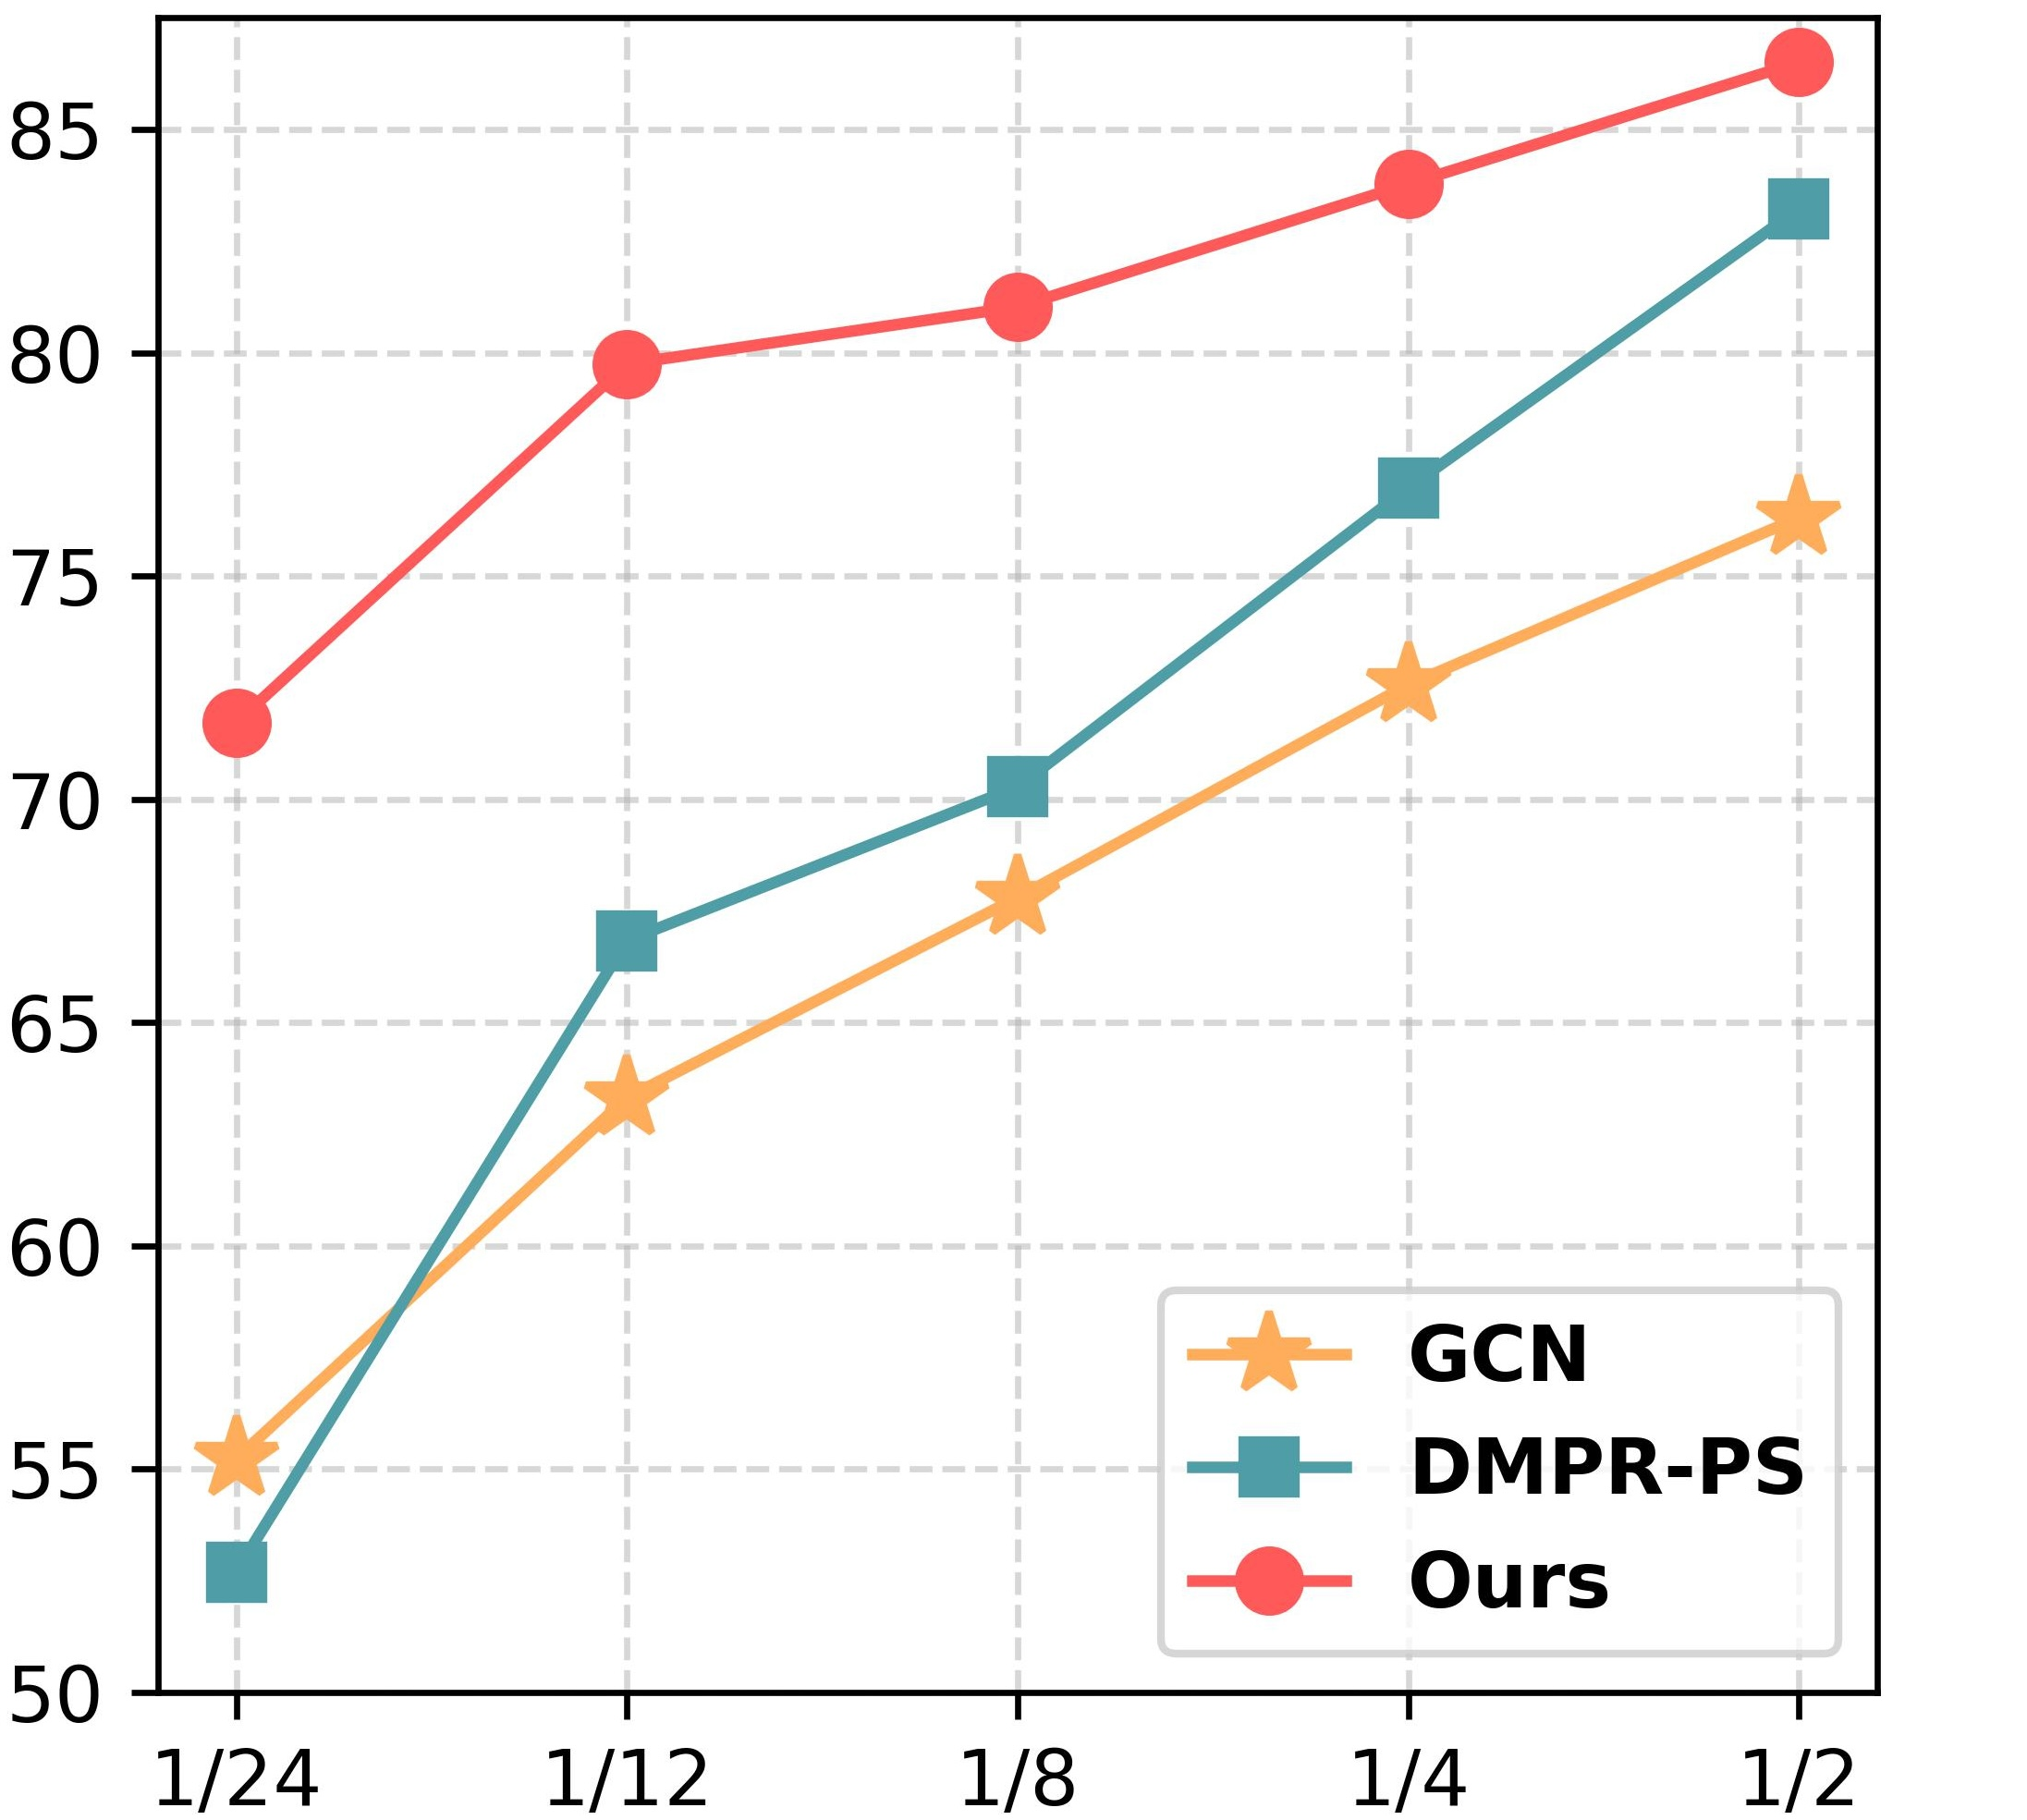
\includegraphics[width=0.43\linewidth]{figures/chp2/curve/curve_s2.jpg}}
    \label{5a}
	  \subfloat[ps2.0]{
        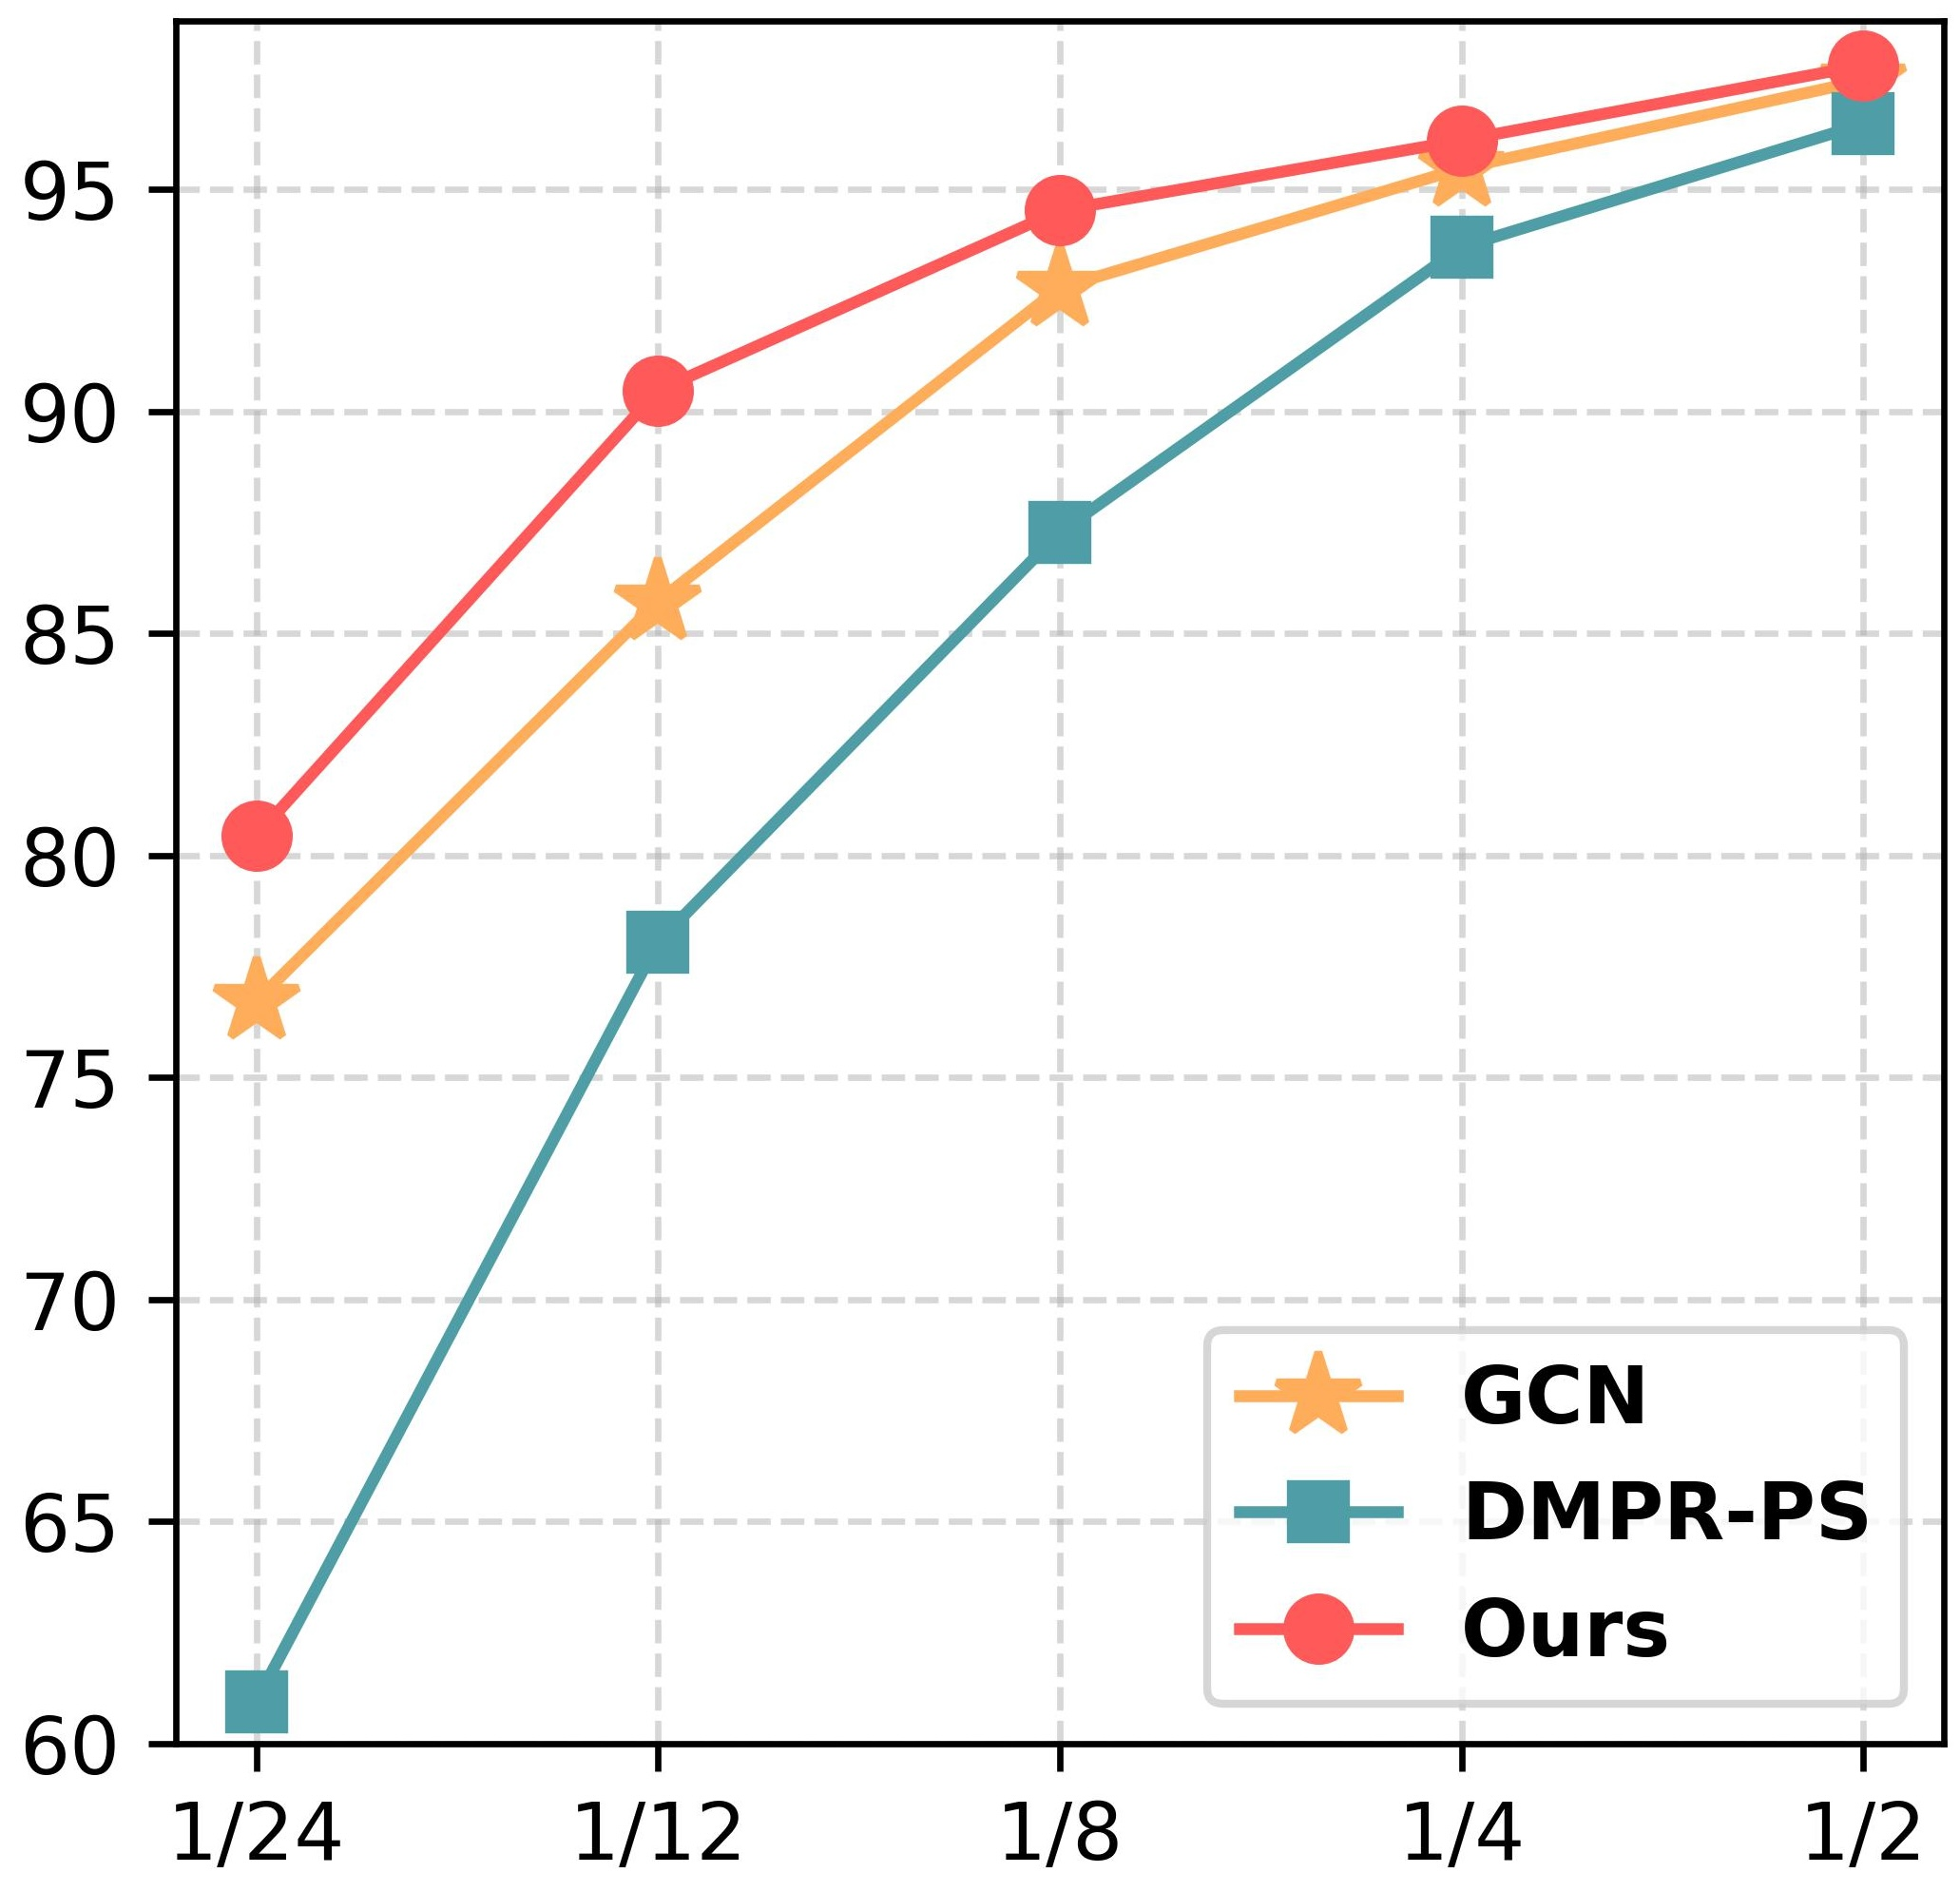
\includegraphics[width=0.4\linewidth]{figures/chp2/curve/curve_s1.jpg}}
    \label{5b}
    \caption{与监督基线相比的改进情况 \\Fig~\ref{fig_curve}~ Improvements over the supervised baseline}
    \label{fig_curve} 
\end{figure}

图\ref{fig_curve}展示了本文方法和监督基线在(a) CRPS-D 和(b) ps2.0上采用不同分区协议的结果。由于CRPS-D数据集相较于ps2.0数据集具有更高的复杂性与真实性，因此本文模型在CRPS-D数据集上相较于监督式基线模型的表现提升更为显著，特别是在标注数据量较少的情况下。所提出的半监督方法能够有效地从CRPS-D数据集中提取更为广泛的特征。 


\subsection{未标记数据有效性分析}

需要说明的是，本文首次提出用于停车位检测的半监督方法，因此直接将其与全监督方法作比较并非完全公平。

\begin{table}[ht]
\centering
\setlength{\tabcolsep}{3mm}
\caption{与近期方法的比较结果 \\
Table~\ref{tab_recent}~Comparison results with recent methods.}
\begin{tabular}{lccccc}
\toprule
    方法 & 标签数 & 图像数 &  Precision & Recall & F1 \\
\midrule
    SAM-PS\cite{zhai2024sam} & 0 & 9827 & 94.29\% & 81.35\% & 87.34\% \\
    \textbf{Ours (1/12)} & \textbf{819} & 9827 & \textbf{95.45\%} & \textbf{91.30\%} & \textbf{93.34\%} \\
\midrule
       DeepPS\cite{zhang2018vision}  & 9827 & 9827 & 98.99\% & 99.13\% & 99.06\% \\
       DMPR-PS\cite{huang2019dmpr} & 9827 & 9827 & 99.42\% & 99.37\% & 99.39\% \\
       VPS\cite{li2020vacant}  & 9827 & 9827 & 99.63\% & 99.10\% & 99.36\% \\
       GCN\cite{min2021attentional}  & 9827 & 9827 & 99.56\% & 99.42\% & 99.49\%\\
       SCCN \cite{zheng2022center}  & 9827 & 9827 & 99.35\% & 99.17\% & 99.26\% \\
       Bui et al.\cite{bui2023one} & 9827 & 9827 &  99.63\% & 99.63\% & 99.63\% \\
       BEV-PolyNet\cite{duan2025bev} & 9827 & 9827 &  99.82\% & 99.65\% & 99.73\% \\
       \textbf{Ours (1/2)} & \textbf{4913}  & 9827 & 98.64\% & 98.07\% & 98.35\%\\
\bottomrule
\end{tabular}
\label{tab_recent}
\end{table}

即便如此，本文仍提供更多与近期方法的对比结果。需注意，这些方法（如SCCN(2020)\cite{zheng2022center}、Bui等人(2023)\cite{bui2023one} 以及SAM - PS(2024)\cite{zhai2024sam}）并非开源，所以本文只能报告其原始论文在ps2.0数据集上的性能。结果如表 \ref{tab_recent} 所示，其中“Ours (1/n)”表示使用\(1/n\)个标签进行训练。

当仅使用\(1/12\)的标签（819个）时，本文的半监督方法性能显著优于现有的自监督方法（SAM-PS\cite{zhai2024sam}）。此外，当使用一半的标签（4913个）时，本文方法获得了与全监督模型（如VPS\cite{li2020vacant}）相当的性能，差异仅约为\(1\%\)。

此外，本节还展示了随着标注数据比例增加，SS-PSD与完全监督模型（本文的基线模型DMPR-PS \cite{huang2019dmpr}）之间的性能差距。如图 \ref{fig_ps} 和 \ref{fig_crps} 所示，当仅有少量标注数据时，SS-PSD的性能始终优于完全监督基线模型。黄色部分表示SS-PSD方法带来的性能提升，随着标注数据量增多，这种性能差距逐渐缩小。这种收益递减现象符合预期，因为一旦有足够的标注数据，利用未标注数据的边际收益便会降低。

    \begin{figure}[!h]
    \centering
    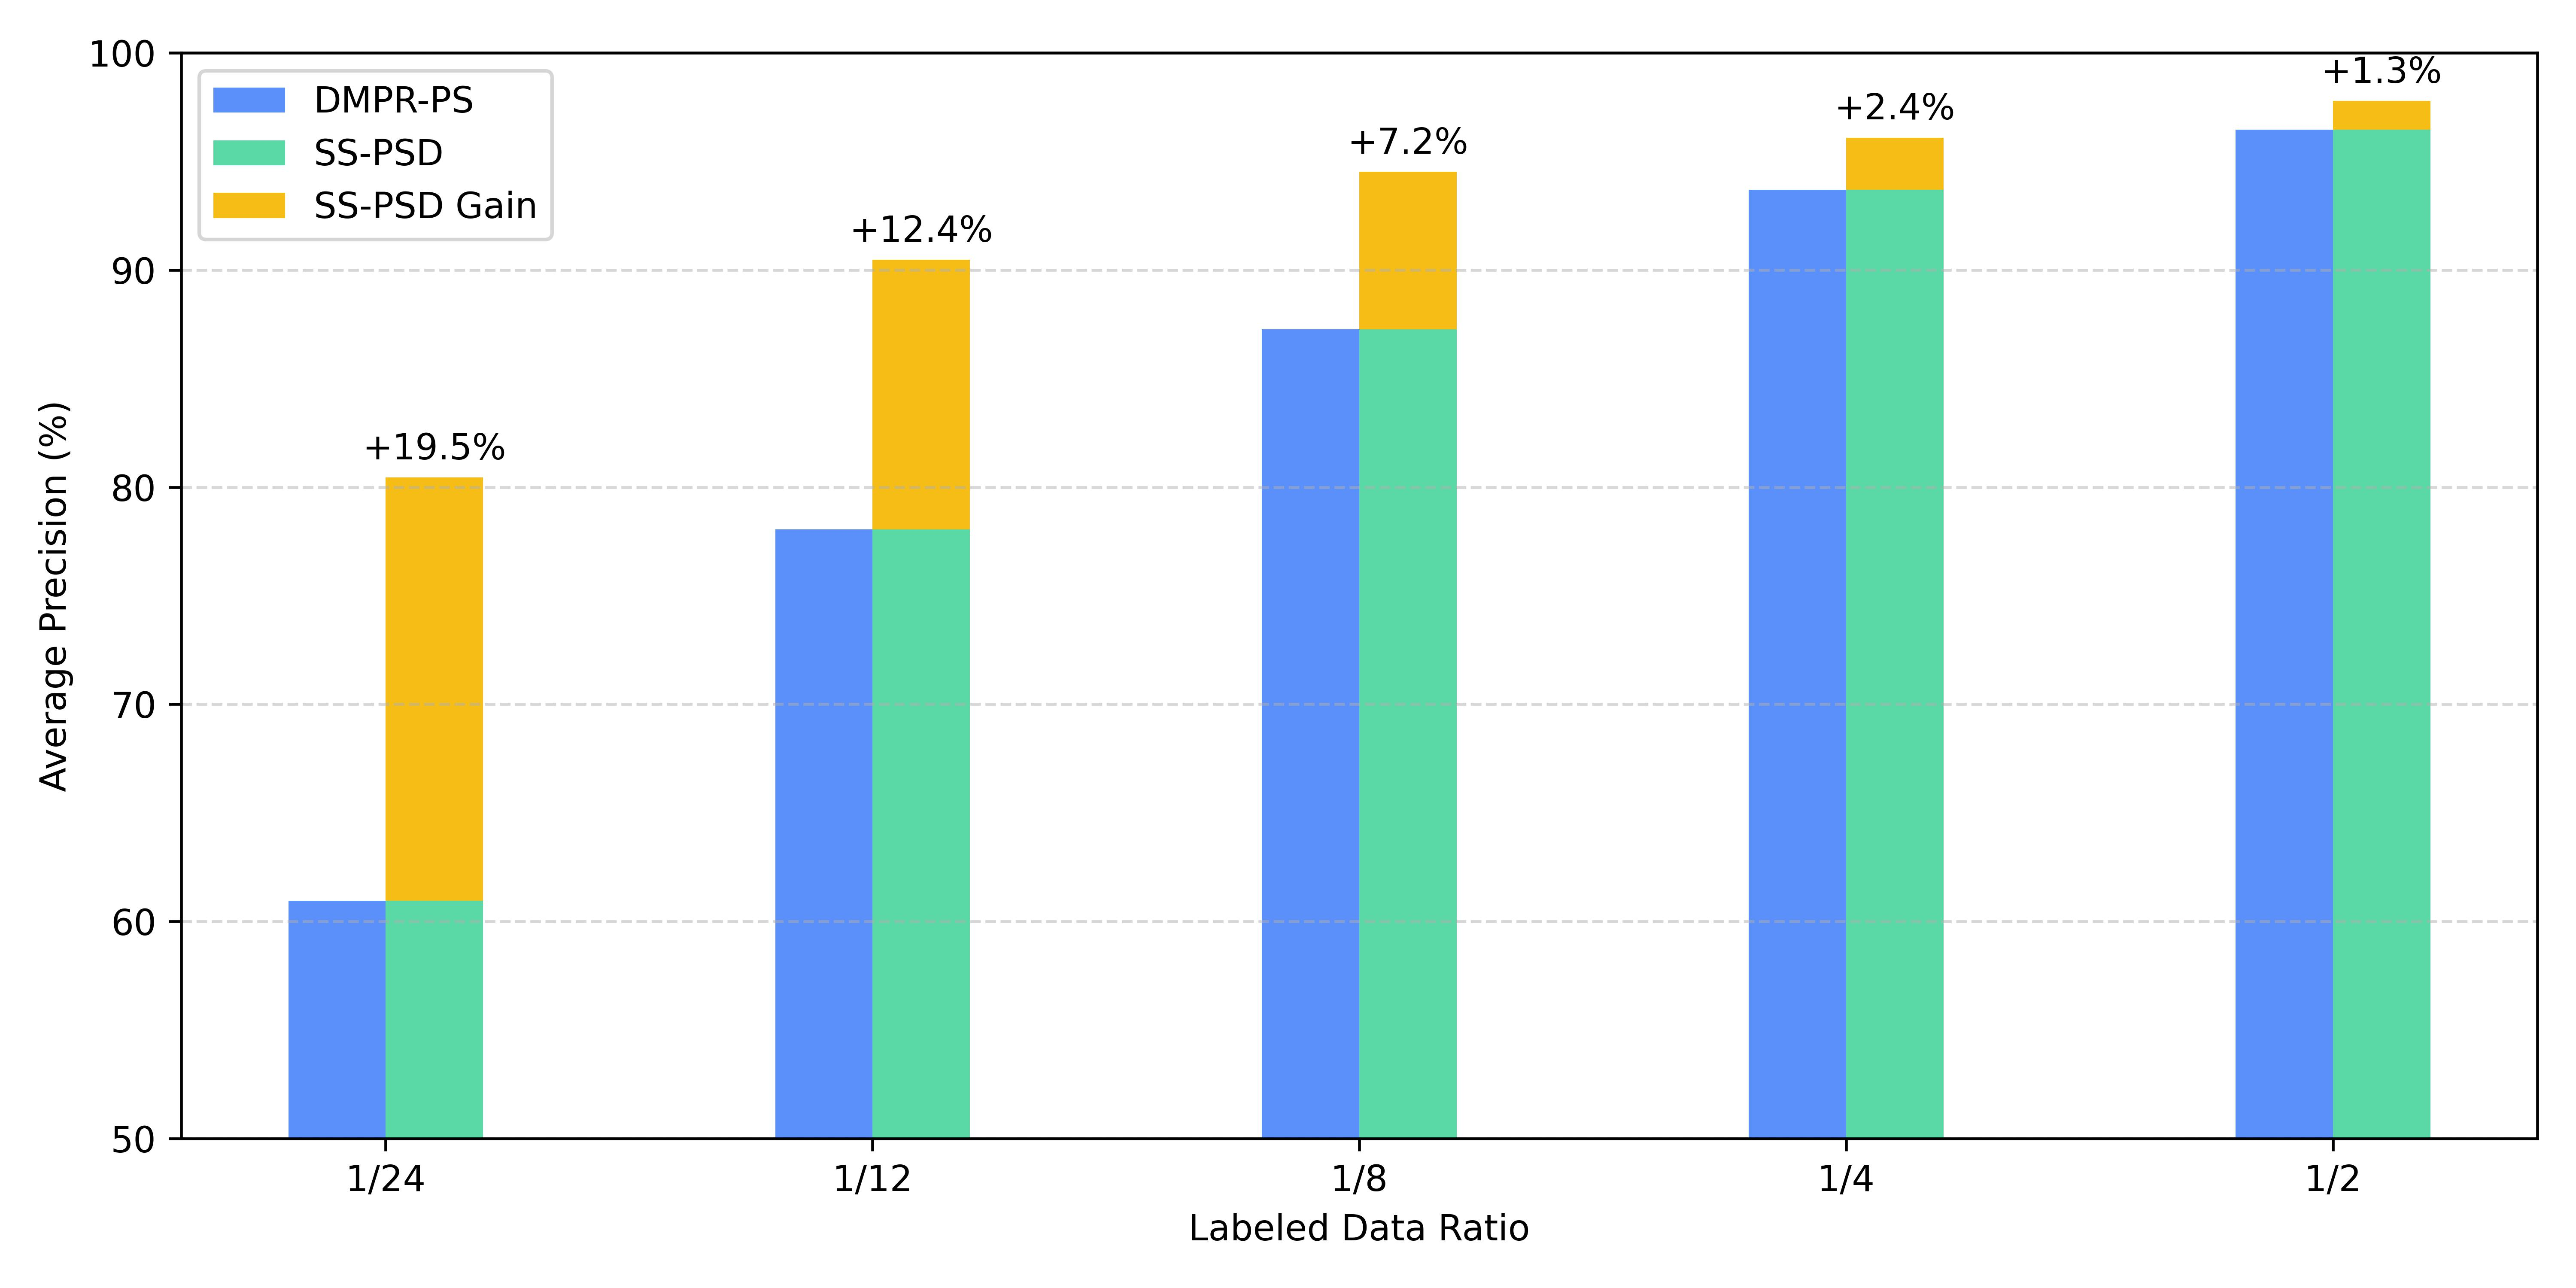
\includegraphics[width=1\linewidth]{figures/chp2/bar/ps.jpg}
    \caption{SS-PSD与DMPR-PS的性能比较（ps2.0数据集） \\Fig~\ref{fig_ps}~ Performance comparison of SS-PSD and DMPR-PS (ps2.0 dataset)}
    \label{fig_ps}
   \end{figure}

    \begin{figure}[!h]
    \centering
    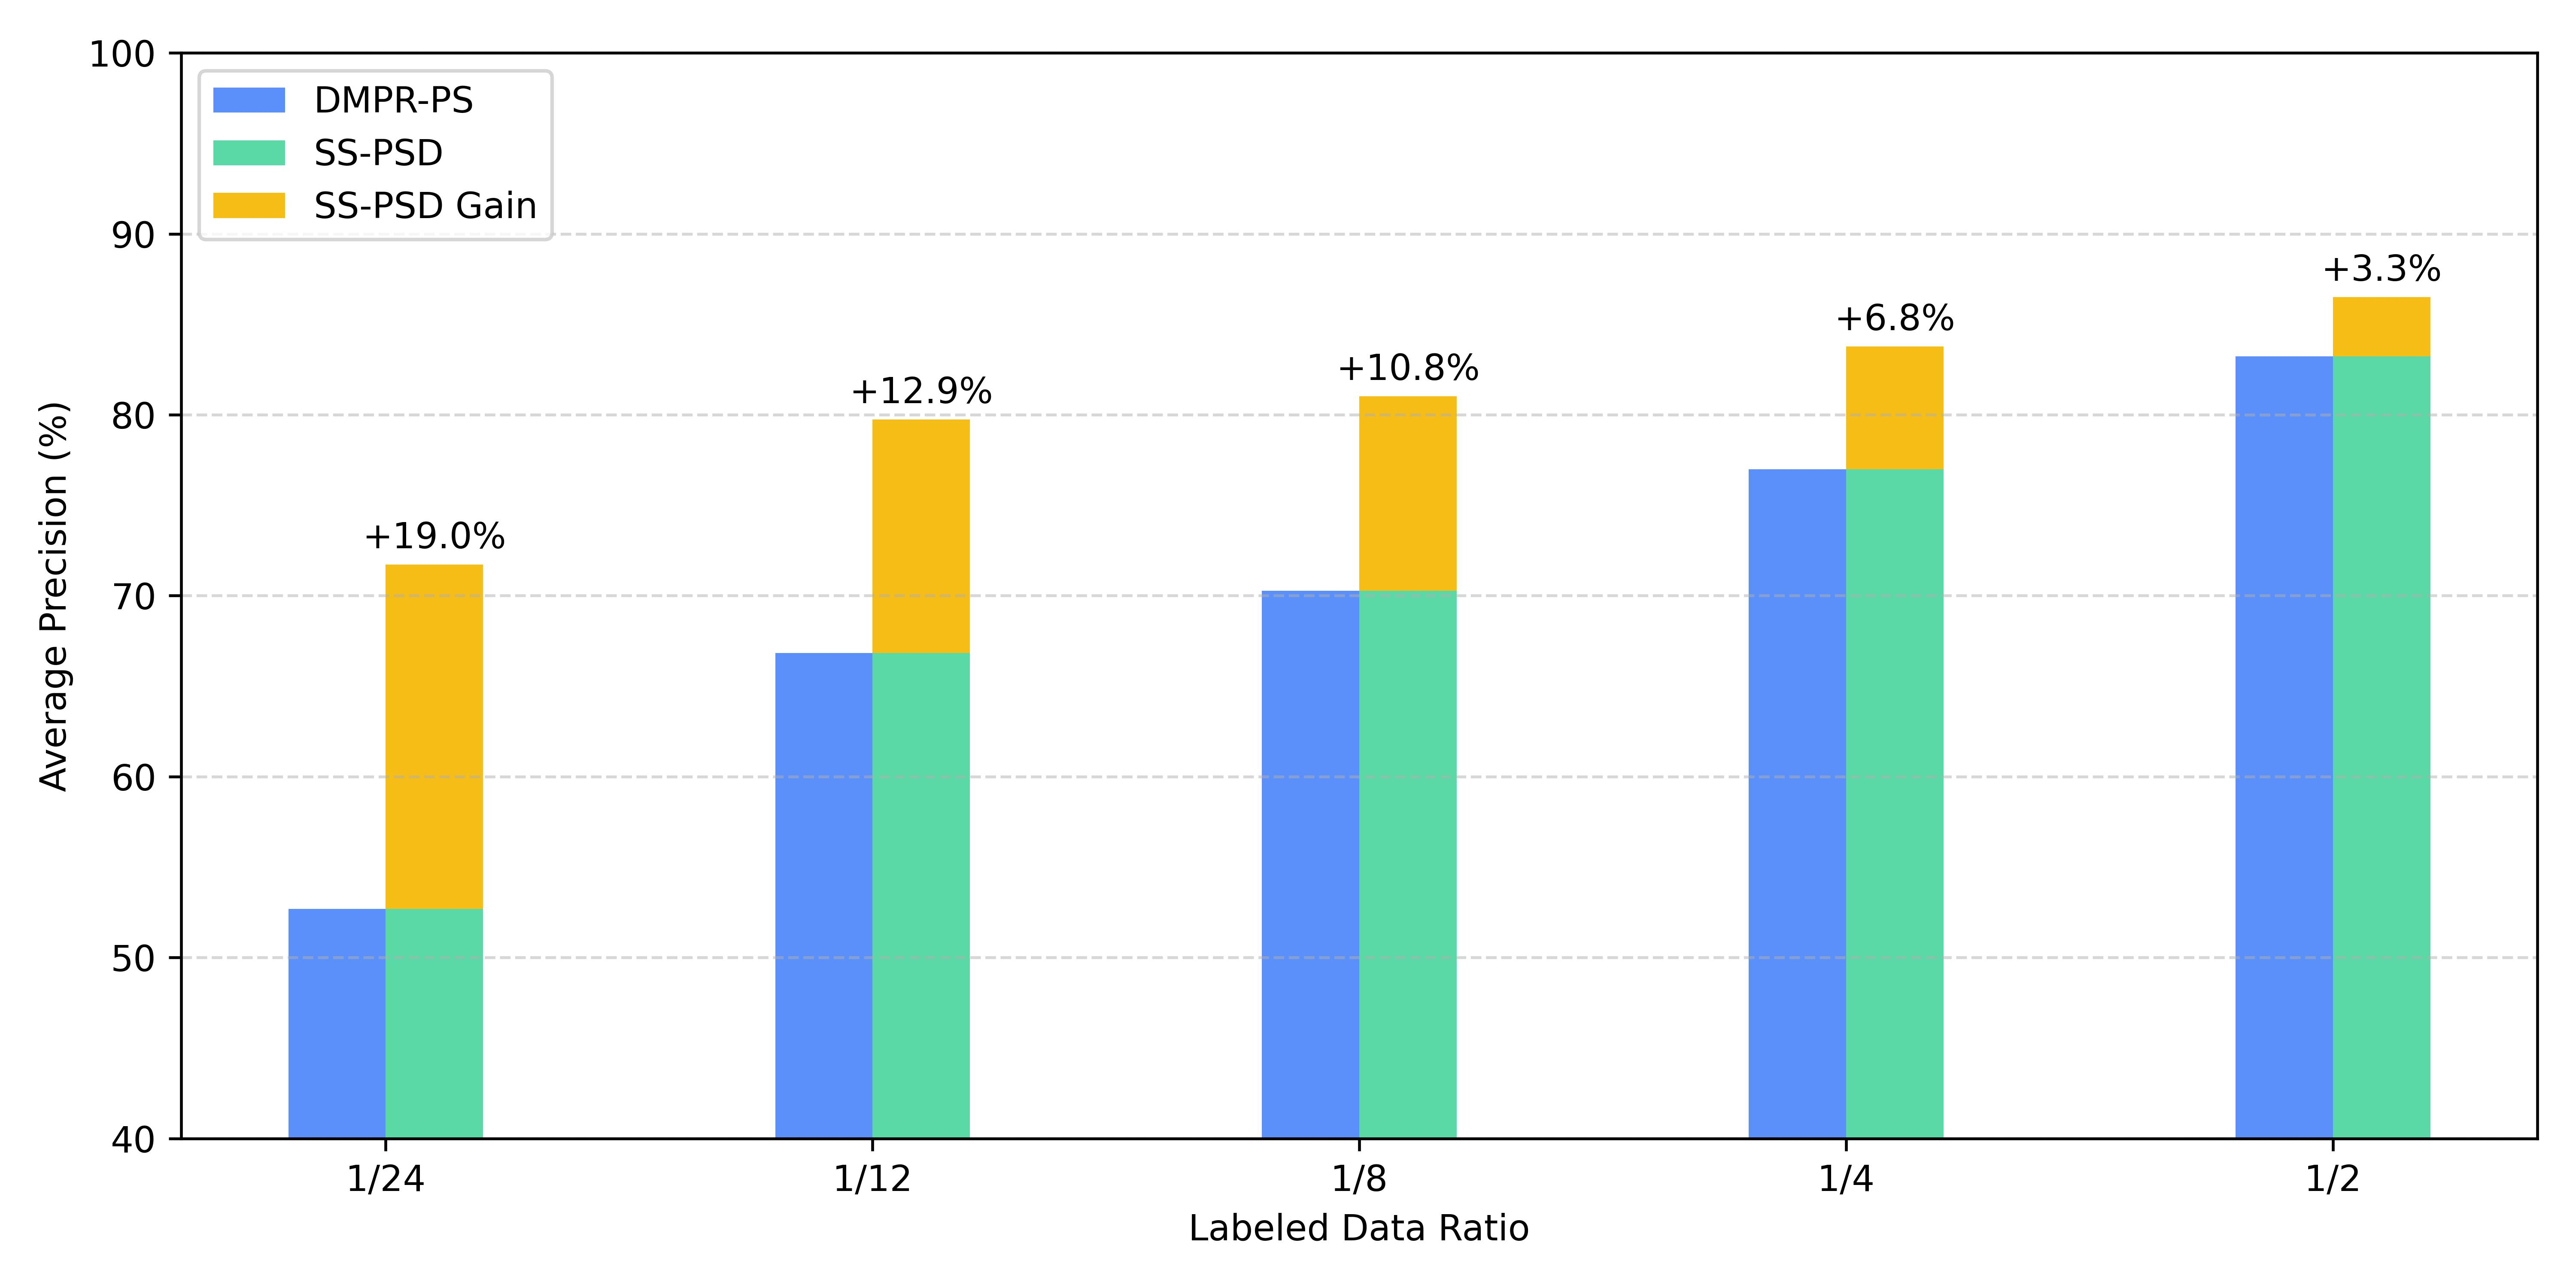
\includegraphics[width=1\linewidth]{figures/chp2/bar/crps.jpg}
    \caption{SS-PSD与DMPR-PS的性能比较（CPRS-D数据集） \\Fig~\ref{fig_crps}~ Performance comparison of SS-PSD and DMPR-PS (CPRS-D dataset)}
    \label{fig_crps}
   \end{figure}

这些结果突出了本文方法在标注数据稀缺场景下的有效性，以及随着监督数据量增加，其可扩展性也得以提升，使其成为标注资源有限的实际应用场景的实用解决方案。 


\subsection{消融实验}
本节探究了置信度引导掩码（CGM）一致性和自适应VAT扰动对所提方法的影响。所有实验均基于CRPS-D数据集展开，标注数据比例设定为1/12。各组成部分的贡献详见表\ref{tab_ab}。本节同时展示了标记点和停车位的检测结果。相较于采用均方误差（MSE）损失的半监督基线MT方法，CGM一致性使停车位检测平均精度（$AP_{parking - slot}$）提升了3.60\%，自适应VAT则可进一步提高0.82\%。

\begin{table}[!h]
\centering
\caption{消融实验结果（1/12标注数据） \\
Table~\ref{tab_ab}~Ablation study using the 1/12 labeled ratio}
\begin{tabular}{cccccc}
\toprule
   有监督基线 & MT & CGM Consistency  & Adaptive-VAT & $AP_{marking-point}$ & $AP_{parking-slot}$ \\
\midrule
    \checkmark  &  &  &  & 72.47\% & 66.84\% \\
     \checkmark & \checkmark &  &  & 78.77\% & 75.33\% \\
     \checkmark & \checkmark & \checkmark &  & 80.86\% & 78.93\% \\
     \checkmark & \checkmark & \checkmark & \checkmark & \textbf{81.59\%} & \textbf{79.75\%} \\
\bottomrule
\end{tabular}
\label{tab_ab}
\end{table}

此外，本节分别针对CGM一致性和Adaptive-VAT进行了消融实验，以进一步验证其有效性。

（1）CGM 一致性

本节深入剖析了各类因素对CGM一致性的影响。首先，去除掩码得到CG一致性，接着去除置信度权重得到C一致性。由表\ref{tab_ablation}可知，对所有单元格施加相同约束以保证一致性，无法取得理想结果（平均精度为55.48\% AP）。然而，借助置信度来指导权重分配，可显著提升结果，而对低置信度区域进行掩码处理，能进一步将结果提升0.71\%。

（2）Adaptive-VAT

若去除Adaptive - VAT的自适应性，其性能会降至 `S-VAT`\cite{tarvainen2017mean}或T-VAT\cite{liu2022perturbed}的水平。
如表\ref{tab_ablation}所示，应用Adaptive-VAT能够获得更优性能，因为它可以在 `S-VAT` 和T-VAT之间自适应地选择更优策略。

\begin{table}[!h]
\centering
\caption{对CGM Consistency和Adaptive-VAT的消融实验 \\
Table~\ref{tab_ablation}~Ablation study of various components on CGM Consistency and Adaptive-VAT}
\setlength{\tabcolsep}{8.0mm}
\begin{tabular}{lcc}
\toprule
  Methods &  $AP_{marking-point}$ & $AP_{parking-slot}$ \\
\midrule
      C consistency &   60.07\% & 54.88\% \\
      CG consistency &   80.75\% & 78.22\% \\
      CGM consistency &  \textbf{81.86\%} & \textbf{78.93\%} \\
\midrule
        S-VAT &   80.97\% & 78.87\% \\
       T-VAT &   81.16\% & 79.53\% \\
        Adaptive-VAT &  \textbf{81.59\%} & \textbf{79.75\%} \\
\bottomrule
\end{tabular}
\label{tab_ablation}
\end{table}

\subsection{超参选择}

本节讨论两个关键超参数的值选择：置信度阈值 ($\tau$) 和干扰强度 ($eps$)。实验均使用 1/12 标注比例在 CRPS-D 数据集上训练。

（1）置信度阈值 ($\tau$)

参考FixMatch\cite{sohn2020fixmatch}的方法（该方法通过选取置信度更高的标签来提升伪标签的准确率），本文设置了较高的阈值（$\tau$ = 0.9）。此外，本文还尝试了将置信度阈值在0到1之间以 0.1 为步长进行变化。如表\ref{tab_confidence}所示，当阈值为0.9时性能最优。 

\begin{table}[!h]
\centering
\caption{不同置信度阈值的实验结果\\
Table~\ref{tab_confidence}~Results of different confidence thresholds.}
    \begin{tabular}{cccc}
    \toprule
    Threshold ($\tau$) & $AP_{marking-point}$ & $AP_{parking-slot}$ & Epochs\\
    \midrule
    0.1 & 81.12\% & 78.81\%	& 36 \\
    0.2	& 81.59\%	& 79.47\%	& 22 \\
    0.3	& 81.28\%	& 79.08\%	& 21 \\
    0.4	& 81.13\%	& 79.34\%	& 23 \\
    0.5	& 81.06\%	& 79.01\%	& 17 \\
    0.6 & 80.75\%	& 79.10\%	& 40 \\
    0.7	& 81.38\%	& 79.50\%	& 23 \\
    0.8	& 80.75\%	& 78.95\%	& 26 \\
    0.9	& \textbf{81.59\%}	& \textbf{79.75\%}	& 22 \\
    \bottomrule
    \end{tabular}
\label{tab_confidence}
\end{table} 

（2）干扰强度 ($eps$)

为证明本文所提Adaptive-VAT算法在各类干扰强度下均能展现优异性能，本文对干扰强度进行了改变，分别采用\(eps\) = 10、1和0.1这几个取值。 

\begin{table}[!h]
\centering
\caption{不同干扰强度的实验结果\\
Table~\ref{tab_eps}~Results of different disturbance intensities}
\begin{tabular}{ccccccc}
\toprule
 & \multicolumn{3}{@{}c@{}}{$AP_{marking-point}$} & \multicolumn{3}{@{}c@{}}{$AP_{parking-slot}$} \\\cmidrule{2-4}\cmidrule{5-7}%
   \multirow{-2}{*}{$eps$}  & S-VAT & T-VAT & Ours & S-VAT & T-VAT & Ours \\
\midrule
    10.0 & 80.89\% & 80.78\% & 81.32\% &79.11\% & 78.89\% & 79.15\%  \\
     1.0 & 80.87\% & 81.04\% & 81.68\% &78.65\% &78.89\% & 79.54\%  \\
     0.1 & 80.97\% & 81.16\% & \textbf{81.59\%} & 78.87\% & 79.53\% & \textbf{79.75\%}  \\
\bottomrule
\end{tabular}
\label{tab_eps}
\end{table}


如表~\ref{tab_eps}所示，与S-VAT和T-VAT相比，本文提出的Adaptive-VAT方法性能更优。基于实验结果，本文最终选择$eps = 0.1$。


\subsection{分场景结果}

表\ref{tab_test}呈现了监督基线方法 (DMPR-PS\cite{huang2019dmpr}) 与本文所提SS-PSD方法在不同场景（对应于CRPS-D数据集的子测试集）下的性能评估情况。该结果基于CRPS-D数据集训练得出，其中标注数据与未标注数据的比例为1/12。无论是在简单场景（如“室内弱光”“室外阴影”），还是复杂场景（如“受损车位”“室外夜晚”），本文模型均展现出更优的性能。停车位检测的可视化结果如图\ref{fig_result}所示。

尤为突出的是，本文的半监督解决方案能够通过有效利用易于获取的未标注数据，显著缓解长尾分布所带来的难题。例如，“室外夜晚”子集的数据规模最小，在监督方案下表现最差，而本文的SS-PSD方法则可大幅提升模型性能。 

\begin{table}[!h]
\centering
\caption{分场景子测试集的实验结果\\
Table~\ref{tab_test}~Evaluation results on the sub-test sets}
\setlength{\tabcolsep}{5.0mm}
\begin{tabular}{lcccc}
\toprule
 \multicolumn{2}{c}{} & \multicolumn{2}{c}{$AP_{parking-slot}\uparrow$} \\ \cmidrule{3-4}%
   \multirow{-2}{*}{场景子集} & \multirow{-2}{*}{图像数} & DMPR-PS$^{*}$ & \textbf{Ours} & \multirow{-2}{*}{提升} \\
\midrule
      室内弱光 & 545  & 74.15\% & 86.68\% & 12.53\%\\
      室内强光 & 786  & 70.00\% & 84.80\% & 14.80\%\\
      阴影 & 1389  & 69.19\% & 81.09\% & 11.90\%\\
      正常日光 & 1703  & 68.06\% & 78.99\% & 10.93\%\\
\midrule
      倾斜车位 & 802  & 61.61\% & 76.79\% & 15.18\%\\
      受损车位 & 302  & 58.90\% & 71.83\% & 12.93\%\\
      雨天 & 323  & 56.07\% & 71.07\% & 15.00\%\\
      夜晚 & 86  & 38.38\% & 63.45\% & \textbf{25.07\%} \\
\bottomrule
\end{tabular}
 \label{tab_test}
\end{table}


\begin{figure}[!h]
\centering
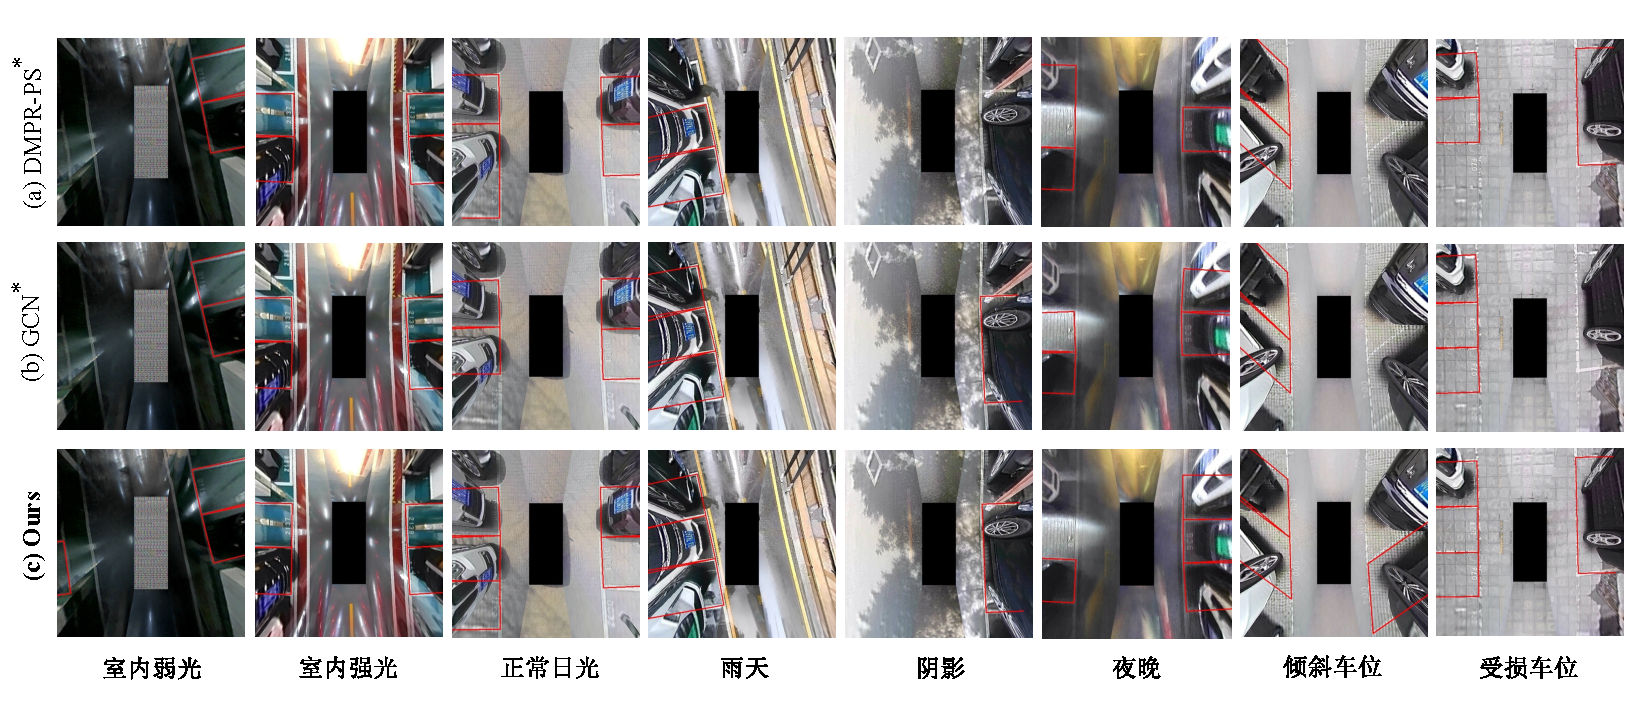
\includegraphics[width=1\textwidth]{figures/chp2/pdf/result.pdf}
\caption{不同场景的可视化结果 \\Fig~\ref{fig_result}~Visualized results of different scenes}
\label{fig_result}
\end{figure}



\section{本章小结}

本章聚焦于复杂真实场景中停车位检测任务面临的数据规模受限以及标注成本高昂问题，构建了一个大规模停车位数据集。该数据集覆盖多光照、多视角以及多停车形式，为后续方法研究搭建了统一的数据基础。此数据集包含在各类天气条件下拍摄的鸟瞰图像，涵盖多种场景。相较于以往数据集，它更具挑战性，不仅规模更大、场景更多样，倾斜停车位比例更高，还包含更多标线损坏的复杂实例。此外，本章提出一种面向停车位检测任务的半监督检测框架，借助教师-学生学习范式，有效运用未标注数据，提升模型的泛化能力与鲁棒性。

本章工作从数据与学习范式两个层面，缓解了停车位检测在复杂场景下的训练瓶颈，为后续基于单帧与多帧建模的检测方法，奠定了坚实的数据与训练基础。 


